\subsection{Cost benefit analyse}
\label{Cost_Ben}
Da vi skulle implementere vores system var det vigtigt for os, at vi valgte den korrekte implementationsstrategi i forhold til, hvor meget gavn brugeren ville få ud af de forskellige løsninger. Vi overvejede derfor hvilken nytte brugerne ville få hvis vi brugte en implementationsmulighed frem for en anden og hvor meget det ville koste os at implementere det. For at få et overblik over, hvordan disse ting forholdt sig til hinanden valgte vi at lave et skema der viste nytten af en implementation kontra omkostninger.

\begin{figure}[h!]
  \centering
    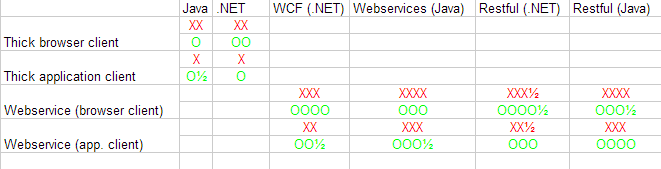
\includegraphics[width=0.5\textwidth]{Appendix/GUI-Prototype/CostBenefit}
  \caption{Tabel over cost/benefit i forhold til de forskellige implementations muligheder}
\label{Cost_Ben}
\end{figure} 

Figur \ref{Cost_Ben} viser vores cost benefit skema over de forskellige implementationsmuligheder. De røde X'er repræsenterer omkostningerne for at implementere den tilsvarende kombination. For at komme frem til omkostningerne af de forskellige implementationsmuligheder tog vi udgangspunkt i hvorvidt vi først skulle tilegne os viden eller om vi allerede havde den fornødende forståelse og således kunne gå i gang med det samme. eksempelvis ville en "Java, Thick browser client" løsning være dyrere end en "Java, Thick application client"løsning da vi ikke ved, hvordan man laver en browser klient i java. Derefter kiggede vi på, hvor meget kode der skulle skrives til de forskellige implementationsmodeller for at kunne få et fungerende system. Eksempelvis er alle Webservice løsningerne dyrere end Thick client løsningerne, da der skal kodes mere, hvis der skal laves en webservice.


De grønne O'er repræsenterer den gavn som brugeren får af den givne implementationsmodel. En af måderne, hvor vi fandt ud af hvor meget gavn de forskellige implementationsmuligheder gav brugeren var at se på, hvor mange platforme der var understøttet.

Eksmepelvis synes vi, at det gav brugeren mere nytte, hvis deres system kunne køre på alle computerere i en browser end hvis man skulle downloade en klient og tjekke om den kunne køre på computeren. Derudover kiggede vi også på, hvor nemt det ville være for brugeren at udvikle videre på systemet, eksempelvis giver implementationsmuligheden "WCF(.NET), Webservice(browser client)" brugeren mulighed for at udvikle en applikation til windows phone da der er en service at kode op imod.

Udfra de måder at vurderer cost benefit på vurderede vi, at den løsning hvor kunden ville få mest gavn var "WCF(.NET), Webservice (browser client)" da det ville give brugeren mulighed for at kunne køre systemet på stort set alle computerere med internet connection og, at de ville være i stand til at lave en mobilapplikation op imod webservicen.



 